\documentclass[12pt]{article}

\usepackage[utf8]{inputenc}
\usepackage[danish]{babel}
\usepackage{latexsym, amsfonts, amssymb, amsthm, amsmath, siunitx, graphicx, pgfplots}
\usepackage[hidelinks]{hyperref}
\usepackage[comma]{numerica}

\sisetup{exponent-product = \cdot,
  output-decimal-marker = {,}}

%Giles Castelles incfig
\usepackage{import}
\usepackage{xifthen}
\usepackage{pdfpages}
\usepackage{transparent}

\newcommand{\incfig}[2][1]{%
  \def\svgwidth{#1\columnwidth}
  \import{../figures/}{#2.pdf_tex}
}

\pdfsuppresswarningpagegroup=1

\setlength{\parindent}{0in}
\setlength{\oddsidemargin}{0in}
\setlength{\textwidth}{6.5in}
\setlength{\textheight}{8.8in}
\setlength{\topmargin}{0in}
\setlength{\headheight}{18pt}

\pgfplotsset{compat=newest}

\pgfplotsset{every axis/.append style={
  axis x line=middle,    % put the x axis in the middle
  axis y line=middle,    % put the y axis in the middle
  axis line style={<->,color=black}, % arrows on the axis
}}

\title{Opgaver til forelæsning 13}
\author{Noah Rahbek Bigum Hansen}
\date{15. Oktober 2024}

\begin{document}

\maketitle

\section*{Opg. 9.5}
A child is pushing a merry-go-round. The angle through which the merry-go-round has turned varies with time according to $\theta (t) = \gamma t + \beta t^3$, where $\gamma = \qty{0,400}{\frac{rad}{s}}$ and $\beta = \qty{0,0120}{\frac{rad}{s^3}}$.

\subsection*{(a)}
Calculate the angular velocity of the merry-go-round as a function of time.
\bigbreak
For at regne vinkelhastigheden differentierer vi blot funktionen for position idet $ \omega(t) = \frac{\mathrm{d}\theta}{\mathrm{d}t}$. Altså har vi at
\[
\omega (t) = \gamma + 3\beta t^2 
.\] 

\subsection*{(b)}
What is the initial value of the angular velocity?
\bigbreak
Sættes $t = 0$ fås
 \[
\omega (0) = \gamma + 3\beta 0^2 = \gamma = \qty{0,400}{\frac{rad}{s}}
.\] 


\subsection*{(c)}
Calculate the instantaneous value of the angular velocity $\omega_z$ at $t = \qty{5,00}{s}$ and the average angular velocity $\omega_{av-z}$ for the time interval $t = \num{0}$ to $t = \qty{5,00}{s}$. Show that $\omega_{av-z}$ is \textit{not} equal to the average of the instantaneous angular velocities at $t = \num{0}$ and $t = \qty{5,00}{s}$, and explain.
\bigbreak
Først regnes $\omega (\qty{5,00}{s})$ som
\[
\omega (\qty{5,00}{s}) = \gamma + 3\beta \left( \qty{5,00}{s} \right) ^2 = \qty{0,400}{\frac{rad}{s}} + 3\cdot \qty{0,0120}{\frac{rad}{s^3}} \left( \qty{5,00}{s} \right)^2 = \qty{1,3}{\frac{rad}{s}}
.\]
For at finde den gennemsnitlige vinkelhastighed benyttes at
\begin{align*}
  \overline{\omega_z} &= \frac{1}{\Delta t} \int_0^{\Delta t} \omega_z \, \mathrm{d}t = \frac{\Delta \theta}{\Delta t} \\
  &= \frac{1}{\Delta t} \left[ \gamma t + \beta t^3 \right]_{t_0}^{t_1} \\
  &= \frac{1}{\Delta t} \left[ \gamma t + \beta t^3 \right]\cdot \Delta t\\
  &= \left[ \qty{0,400}{\frac{rad}{s}} + \qty{0,0120}{\frac{rad}{s^3}} \left( \qty{5,00}{s} \right) ^2 \right]  \\
  &= \qty{0,700}{\frac{rad}{s}} \\
.\end{align*}

\section*{Opg. 9.15}
A high-speed flywheel in a motor is spinning at \qty{500}{RPM} when a power failure suddenly occurs. The flywheel has mass \qty{40,0}{kg} and diameter \qty{75,0}{cm}. The power is off for \qty{30,0}{s}, and during this time the flywheel slows due to friction in its axle bearings. During the time the power is off, the flywheel makes 200 complete revolutions.


\subsection*{(a)}
At what rate is the flywheel spinning when the power comes back on?
\bigbreak
Vi får givet at
\begin{align*}
  \omega_{0z} &= \qty{500}{RPM} \\
  &= \frac{\qty{500}{RPM}}{\qty{60}{\frac{s}{min}}} \\
  &= \qty{8,33}{\frac{rev}{s}}
\end{align*}
I de $t = \qty{30,0}{s}$, hvor strømmen er gået bevæger \textit{flywheel}'et sig
\[
\theta - \theta_0 = \qty{200}{rev}
.\] 
Idet vi antager konstant vinkelacceleration under strømafbrydelsen har vi at
\[
  \theta - \theta_0 = \frac{1}{2}\left( \omega_{0z} + \omega_z \right)t
.\] 
Heri kan $\omega_{0z}$ isoleres så vi får at
\[
\omega_{z} = \frac{2\left( \theta - \theta_{0} \right)}{t} - \omega_{0z} = \frac{2\cdot \left( \qty{200}{rev} \right)}{\qty{30,0}{s}} - \qty{8,33}{\frac{rev}{s}} = \qty{5,00}{\frac{rev}{s}} 
.\] 

\subsection*{(b)}
How long after the beginning of the power failure would it have taken the flywheel to stop if the power had not come back on, and how many revolutions would the wheel have made during this time?
\bigbreak
Vi har
\[
\alpha = \frac{\omega_z - \omega_{0z}}{t} = \frac{\qty{5,00}{\frac{rev}{s} - \qty{8,33}{\frac{rev}{s}}}}{\qty{30,0}{s}} = \qty{-0,111}{\frac{rev}{s^2}}
.\] 
Vi bruger at
\[
\omega_z  - \omega_{0z} = \alpha t \implies t = \frac{\omega_z - \omega_{0z}}{\alpha} = \frac{\qty{0}{\frac{rev}{s}} - \qty{8,33}{\frac{rev}{s}}}{\qty{-0,111}{\frac{rev}{s^2}}} = \qty{75,0}{s}
.\] 


\section*{Opg. 9.20}
A compact disc (CD) stores music in a coded pattern of tiny pits \qty{e-7}{m} deep. The pits are arranged in a track that spirals outward toward the rim of the disc; the inner and outer radii of this spiral are \qty{25,0}{mm} and \qty{58,0}{mm}, respectively. As the disc spins inside a CD player, the track is scanned at a constant linear speed of \qty{1,25}{m/s}.

\subsection*{(a)}
What is the angular speed of the CD when the innermost part of the track is scanned? The outermost part of the track?
\bigbreak
Vi har at
\[
  v = r_0 \cdot \omega_{inner} \implies \omega_{inner} = \frac{v}{r_0} = \frac{\qty{1,25}{\frac{m}{s}}}{\qty{25,0}{mm}} = \qty{50}{\frac{rad}{s}}
.\]
Og
\[
v = r_1 \cdot \omega_{outer} \implies \omega_{outer} = \frac{v}{r_1} = \frac{\qty{1,25}{\frac{m}{s}}}{\qty{58,0}{mm}} = \qty{21,55}{\frac{rad}{s}} 
.\] 

\subsection*{(b)}
The maximum playing time of a CD is \qty{74,0}{min}. What would be the length of the track on such a maximum-duration CD if it were stretched out in a straight line?
\bigbreak
Vi har at
\[
s = v \cdot t \implies s = \qty{1,25}{\frac{m}{s}} \cdot \qty{74,0}{min} = \qty{5550}{m} = \qty{5,50}{km} 
.\] 

\subsection*{(c)}
What is the average angular acceleration of a maximum-duration CD during its \qty{74,0}{min} playing time? Take the direction of rotation of the disc to be positive.
\bigbreak
Gennemsnitshastigheden af CD-afspilleren er gennemsnittet af dens starthastighed og dens begyndelseshastighed. Altså har vi at
\[
\overline{\omega} = \frac{\Delta \omega}{\Delta t} = \frac{\qty{21,55}{\frac{rad}{s}} - \qty{50,0}{\frac{rad}{s}}}{\qty{74,0}{min}} = \qty{6,41e-3}{\frac{rad}{s}}
.\] 
  


\section*{Opg. 9.22}
You are to design a rotating cylindrical axle to lift \qty{800}{N} buckets of cement from the ground to a rooftop \qty{78,0}{m} above the ground. The buckets will be attached to a hook on the free end of a cable that wraps around the rim of the axle; as the axle turns, the buckets will rise.

\subsection*{(a)}
What should the diameter of the axle be in order to raise the buckets at a steady \qty{2,00}{cm/s} when it is turning at \qty{7,5}{RPM}?
\bigbreak
For at kriteriet er opfyldt må det gælde at
\[
v = \omega \cdot r \implies r = \frac{v}{\omega} = \frac{\qty{2,00}{\frac{m}{s}}}{\qty{7,5}{\frac{rev}{min}}} = \qty{2,55}{cm}
.\] 

\subsection*{(b)}
If instead the axle must give the buckets an upward acceleration of \qty{0,400}{m/s^2}, what should the angular acceleration of the axle be?
Vi har at
\[
a = r\alpha \implies \alpha = \frac{a}{r} = \frac{\qty{0,400}{\frac{m}{s^2}}}{\qty{2,55}{cm}} = \qty{15,7}{\frac{rad}{s}}
.\] 


\section*{Opg. 9.58}
A uniform disk with radius $R = \qty{0,400}{m}$ and mass \qty{30,0}{kg} rotates in a horizontal plane on a frictionless vertical axle that passes through the center of the disk. The angle through which the disk has turned varies with time according to $\theta(t) = \left( \qty{1,10}{\frac{rad}{s}} \right)t + \left( \qty{6,30}{\frac{rad}{s^2}} \right)t^2$. What is the resultant linear acceleration of a point on the rim of the disk at the instant when the disk has turned through \qty{0,100}{rev}
\bigbreak
Først findes antallet af radianer som \qty{0,100}{rev} svarer til
\[
  \qty{0,100}{rev} = 2\pi \unit{\frac{rad}{rev}} \cdot \qty{0,100}{rev} = \qty{0,6283}{rad}
.\] 
Dernæst findes tidspunktet, $t_{0}$, hvor disken har drejet $\theta = \qty{0,100}{rev}$
\[
t = \frac{\qty{-1,10}{\frac{rad}{s}} \pm \sqrt{\left( \left( \qty{1,10}{\frac{rad}{s}} \right)^2 + 4\cdot \qty{6,30}{\frac{rad}{s^2}} \cdot \qty{0,6283}{rad} \right)}}{2\cdot \qty{6,30}{\frac{rad}{s^2}}} = \qty{0,24}{s} 
.\] 
Vi har
\[
\omega = \gamma + 2\beta t \implies \alpha = 2 \beta
.\] 
Den tangentielle acceleraiton er givet som
\[
a_{tan} = r \alpha = 2r \beta = 2 \cdot  \qty{0,400}{m} \cdot \qty{6,30}{\frac{rad}{s^2}} = \qty{5,04}{\frac{m}{s^2}} 
.\] 
Og den radielle er givet som
\[
a_{rad} = r\omega^2 = r \left( \gamma + 2\beta t \right)^2 = \qty{0,400}{m} \left( \qty{1,10}{\frac{rad}{s}} + 2\cdot  \qty{6,30}{\frac{rad}{s}} \cdot \qty{0,24}{s}\right)^2 = \qty{5,48}{\frac{m}{s^2}}
.\] 
Dermed er den samlede acceleration
\[
a = \sqrt{a_{tan}^2 + a_{rad}^2}  = \sqrt{\left( \qty{5,04}{\frac{m}{s^2}} \right)^2 + \left( \qty{5,48}{\frac{m}{s^2}} \right)^2}  ) = \qty{7,45}{\frac{m}{s^2}} 
.\] 

\section*{Opg. 9.59}
A circular saw blade with radius \qty{0,120}{m} starts from rest and turns in a vertical plane with a constant angular acceleration of \qty{2,00}{rev/s^2}. After the blade has turned through \qty{155}{rev}, a small piece of the blade breaks loose from the top of the blade. After the piece breaks loose, it travels with a velocity that is initially horizontal and equal to the tangential velocity of the rim of the blade. The piece travels a vertical distance of \qty{0,820}{m} to the floor. How far does the piece travel horizontally, from where it broke off the blade until it strikes the floor?
\bigbreak
Først regnes den tangentielle hastighed af fragmentet idet det brækker af. Dette gøres ved hjælp af formlen
\[
  \omega_z = \sqrt{2\alpha_z\left( \theta - \theta_0 \right)} \implies \qty{2,00}{\frac{rev}{s^2}\left( \qty{155}{rev}\cdot 2\pi \frac{rad}{rev} \right) = \qty{44,1337}{\frac{rad}{s}}
}
.\] 
Så
\[
v_0 = r\omega = \qty{0,120}{m} \cdot \qty{44,1337}{\frac{rad}{s}} = \qty{5,296}{\frac{m}{s}}
.\] 
Dernæst findes tiden det tager fragmentet at falde under konstant acceleration
\[
y = \frac{1}{2}g\cdot t \implies t = \sqrt{\frac{2y}{g}} = \sqrt{\frac{2\cdot \qty{0,820}{m}}{\qty{9,81}{\frac{m}{s^2}}}} =\qty{0,4089}{s} 
.\] 
Og den vandrette afstand som dette tilsvarer er
\[
x = v_0 \cdot t = \qty{5,296}{\frac{m}{s}}\cdot \qty{0,4089}{s} = \qty{2,1655}{m} 
.\]

\section*{Opg. 9.61}

\begin{figure} [ht]
  \centering
  \caption{}
  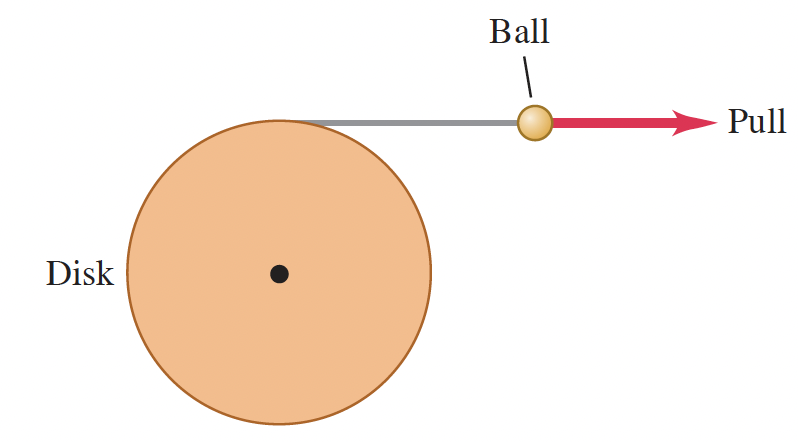
\includegraphics[width=0.5\linewidth]{../figures/P9_61.png}
  \label{fig:P9_61}
\end{figure}

A disk of radius \qty{25,0}{cm} is free to turn about an axle perpendicular to it through its center. It has very thin but strong string wrapped around its rim, and the string is attached to a ball that is pulled tangentially away from the rim of the disk (\textbf{\autoref{fig:P9_61}}). The pull increases in magnitude and produces an acceleration of the ball that obeys the equation $a(t) = At$, where $t$ is in seconds and $A$ is a constant. The cylinder starts from rest, and at the end of the third second, the ball’s acceleration
is \qty{1,80}{m/s^2}.


\subsection*{(a)}
Find $A$.
\bigbreak
Vi har at
\[
a_1 - a_0 = A(t_1 - t_0) \implies A = \frac{a_1}{t_1} = \frac{\qty{1,80}{\frac{m}{s^2}}}{\qty{3,0}{s}} = \qty{0,60}{\frac{m}{s^3}}
.\] 

\subsection*{(b)}
Express the angular acceleration of the disk as a function of time.
\bigbreak
Vinkelaccelerationen er givet som
\[
\alpha\cdot r = a \implies \alpha (t) = \frac{A}{r}t = \frac{\qty{0,60}{\frac{m}{s^3}}}{\qty{25}{cm}}t = \qty{2,40}{\frac{rad}{s^3}}t
.\] 


\subsection*{(c)}
How much time after the disk has begun to turn does it reach an angular speed of \qty{15,0}{rad/s}
\bigbreak
For at finde vinkelhsatigheden integreres udtrykket for vinkelacceleration fundet ovenfor
\[
  \omega(t) = \int \alpha(t) \, \mathrm{d}t = \frac{1}{2}\frac{A}{r}t^2 \implies t = \sqrt{\frac{2\omega(t)\cdot r}{A}} = \sqrt{\frac{2\cdot \qty{15,0}{\frac{rad}{s}}\cdot \qty{25}{cm}}{\qty{0,60}{\frac{m}{s^3}}}} = \qty{3,54}{s}
.\] 



\subsection*{(d)}
Through what angle has the disk turned just as it reaches \qty{15,0}{rad/s}?
\bigbreak
For at finde en funktion for vinkelen integreres vinkelhastigheden så vi får at
\[
\omega(t) = \int \omega(t) \, \mathrm{d}t = \frac{1}{6}\frac{A}{r}\cdot t^3 = \frac{1}{6}\cdot \qty{2,40}{\frac{rad}{s^2}}\cdot t^3 
.\]
Sættes tiden ind fås
\[
\omega(\qty{3,54}{s}) = \frac{1}{6}\cdot \qty{2,40}{\frac{m}{s^2}}\cdot (\qty{3,54}{s})^3 = \qty{17,7}{rad}
.\] 
  


\end{document}
